\chapter{Fundamentos}\label{cap:Fundamentos}

Este capítulo tem como objetivo apresentar a parte histórica e teórica deste trabalho. A revisão de literatura fica a cargo do conteúdo histórico, descrevendo assim uma linha temporal do tema deste TCC. Na fundamentação teórica, serão descritos de forma clara as teorias mais importantes e necessárias para a realização do projeto, como por exemplo as técnicas de modelagem de sistemas e projeto do controlador ótimo.

\section{Revisão de Literatura}

Segundo \cite{Ogata}, trabalhos importantes como de Minorsky, Nyquist e Hazen, datados entre as décadas de 20 e 30, contribuíram para o progresso da teoria de controle. Minorsky, em 1922, trabalhou com pilotagem de embarcações utilizando controladores automáticos e demonstrou por meio de equações diferenciais a estabilidade do sistema. Em 1932, Nyquist desenvolveu um procedimento no qual determina a estabilidade de sistemas em malha fechada com base na resposta em malha aberta. E Hazen, em 1934, introduziu o termo \textit{servomecanismos} para sistemas de controle de posição e analisou o projeto de servomecanismos a relé.

No século XX, acontecimentos como a Segunda Guerra Mundial estimularam as pesquisas em sistemas de controle. No final dos anos 50, a teoria de controle já era bastante consolidada, sendo que o carro chefe era o método que utilizavam a resposta em frequência e com muitas aplicações industriais, como por exemplo: a utilização de controladores PID para o controle de pressão, temperatura, etc. Os métodos de resposta em frequência e do lugar das raízes, os quais são a base da teoria clássica de controle, conduziram os sistemas que são estáveis e satisfatórios para um determinado conjunto de condições. Esses sistemas são aceitáveis, porém não são ótimos no sentido literal do termo. 

Entre as décadas de 60 e 80, segundo \cite{Ogata}, o controle ótimo de sistemas determinísticos, controle adaptativo e de aprendizagem foi altamente pesquisado. Diferentemente da teoria clássica, estes métodos se enquadram na teoria de controle moderno. Essa teoria se baseia no domínio do tempo em sistemas de equações diferenciais. Como vantagem, temos que essa teoria simplificou a realização de projetos de sistemas de controle já que se baseia no modelo de um sistema de controle real. Em contrapartida, a estabilidade é sensível ao erro entre o sistema real e do seu modelo tal como na teoria clássica. Dessa forma, quando o controlador projetado for aplicado no sistema, o mesmo poderá ficar instável devido principalmente ao erro de modelagem. Esse problema é solucionado estabelecendo uma série de possíveis erros no sistema para depois projetar o controlador. Sendo assim, se o erro estiver dentro da predição o sistema será sempre estável. A essa metodologia de projeto baseado nesse princípio é chamado teoria do controle robusto.

%Como vantagem, temos que essa teoria simplificou o projeto de sistemas de controle, já que se baseia no modelo de um sistema de controle real. Em contrapartida, a estabilidade é sensível ao erro entre o sistema real e do seu modelo. Dessa forma, quando o controlador projetado for aplicado no sistema, o mesmo poderá ficar instável. 

%Um dos sistemas clássicos de controle que há na literatura, é o pêndulo invertido. Este sistema possui uma única entrada e várias saídas. Dessa maneira, tratá-lo com técnicas de controle moderno tende a facilitar a estabilidade do mesmo. 

Em \cite{Ooi:03} a técnica utilizada para o controle do pêndulo foi o LQR. Também desenvolveu-se  um controlador por alocação de polos para a estabilização do sistema. Dessa forma, foi capaz realizar a comparação entre esses dois métodos e saber qual dos dois foi mais eficaz. Pelas simulações concluiu-se que os dois métodos atenderam, com ressalva de que o controlador LQR ofereceu maior confiabilidade.

A técnica \textit{PID Backstepping}, que é não linear, foi  utilizada por \cite{PIDBack:10} para controlar um pêndulo invertido sobre duas rodas (PIDR). Essa técnica consiste basicamente em uma estrutura de controle que possui três malhas de controle, sendo elas: 1) a malha principal, desenvolvida a partir da técnica não linear \textit{backstepping} que manterá o pêndulo em equilíbrio; 2) a segunda malha que utiliza um PD para controlar a posição do robô e; 3) um controlador PI para o controle de movimentação.

Em \cite{Junfeng:11} novamente é feito uma comparação entre o controlador ótimo LQR com o controlador por alocação de polos. Contudo, neste artigo, conclui-se que o \textit{overshoot} foi menor por meio da técnica de alocação de polos e que o tempo de estabilização foi quase comparável ao do LQR. 

No artigo de \cite{Juang:13}, os autores propuseram a desenvolver um protótipo utilizando o Arduino como microcontrolador e a implementação de duas técnicas de controle, sendo elas o PID e LQR na forma de PI-PD. Os resultados obtidos deixam bem claro que a técnica PI-PD foi muito mais eficaz em todos sentidos do que a utilização pura do PID. Como concluído, a estabilização por PID é marginal e as oscilações angulares excedem o limite máximo de torque que os motores podem oferecer. Já no PI-PD ou LQR a estabilidade é alcançada e ainda o controlador é capaz de compensar o desalinhamento do CG, fazendo com que o robô retorne para a posição angular desejada.

Em \cite{Paula:14}, o autor utilizou duas técnicas de controle discreto, LQR com ação integral e alocação de polos. A primeira técnica utilizada teve como objetivo a estabilização do pêndulo e a segunda o controle de velocidade dos motores. A técnica de alocação de polos além de realizar o controle dos motores, teve como objetivo interfacear o controle de ângulo e o sinal enviado para os motores. 

Por último, \cite{Alves:18}, além de projetar um controlador LQR, apresenta duas técnicas de linearização, sendo elas: a jacobina e a por realimentação. A modelagem do sistema baseou-se na equação Lagrangiana e após encontrar as equações de movimento, passou-se as mesmas para o Espaço de Estados. Os resultados obtidos foram satisfatório, contudo, ao sofrer interferências, como distúrbio e ruídos o sistema passa a ser mais oscilante.

Como dissertado acima, há vários trabalhos com diferentes resultados para o mesmo tema. Por se tratar de um sistema naturalmente instável, não linear e bastante complexo para controlar, é lógico que haverão trabalhos com resultados distintos. Entretanto, quando há domínio de um determinado assunto, é possível transformar os resultados teóricos em algo para a sociedade, como por exemplo o \textit{Segway}, que é um veículo elétrico de transporte humano e seu funcionamento é baseado no pêndulo invertido sobre duas rodas.

O \textit{Segway}, visto na Figura \ref{fig:revisao_segway}, inventado por Dean Karmen e revelado em dezembro de 2001 tem o funcionamento idêntico ao do pêndulo invertido, com adição que o mesmo está sobre duas rodas. A função básica deste veículo é o transporte de uma única pessoa. O sistema entende que deve-se locomover para frente ou mesmo frear, devido à inclinação que o passageiro impõe sobre o veículo. Hoje em dia, existem vários modelos e cada um com uma especificação diferente um do outro.
\begin{figure}[H]
    \centering
    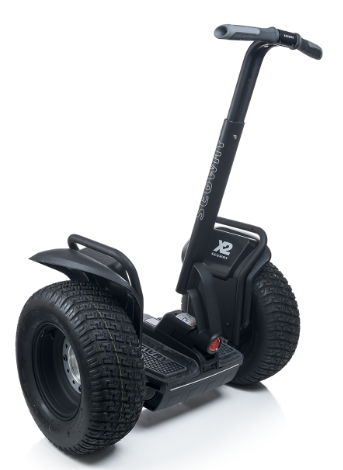
\includegraphics[scale=0.5]{Fundamentos/Segway}
    \caption{Segway X2 SE
    \citep{Segway}.}
    \label{fig:revisao_segway}
\end{figure}

Logo abaixo, segue uma série de trabalhos similares a este aqui proposto. Será descrito de forma breve um pouco sobre os trabalhos em si e a estratégia de controle utilizada, bem como a apresentação da planta física construída.

\subsection{Trabalhos Similares}

O trabalho de \cite{CCEL:17} consistiu na construção de um protótipo projetado por meio de um \textit{software} CAD, visto na Figura (\ref{fig:estadoArte_REF1}), e no desenvolvimento de um sistema de controle para esse projeto. Os autores se engajaram em controlar o sistema com um controlador PID, obtendo seus coeficientes por meio do método de sintonização de \textit{Ziegler-Nichols}. Como sensor utilizaram a placa MPU6050, que possui embutida na mesma o giroscópio e acelerômetro. Contudo, se faz necessário a fusão dos sinais provenientes desses dois sensores para obtenção de uma maior confiabilidade e certeza da medição. Sendo assim, os autores optaram por utilizar o filtro complementar, que nada mais é do que um filtro de média. 
\begin{figure}[H]
    \centering
    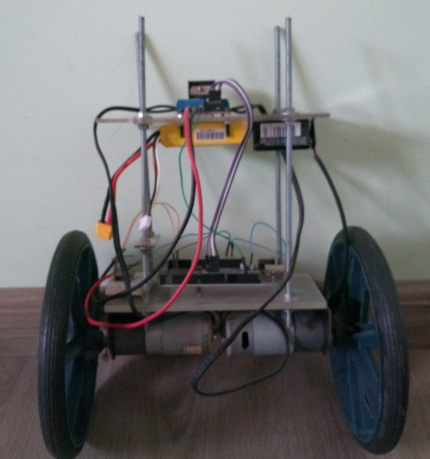
\includegraphics[scale=0.6]{EstadoArte/REF1}
    \caption{Protótipo Pêndulo Invertido
    \citep{CCEL:17}.}
    \label{fig:estadoArte_REF1}
\end{figure}

O artigo de \cite{JVM:17} teve como objetivo a identificação e o controle de um veículo do tipo Segway para fins educacionais. Dessa maneira, o autor dividiu o artigo em partes como: o sistema eletrônico e mecânico, linearização do modelo matemático e discretização, implementação de filtros para a leitura dos sinais provindo do acelerômetro e giroscópio, identificação do sistema e a implementação de um controlador PD (Proporcional-Derivativo), sendo que seus coeficientes foram obtidos por meio de inspeção gráfica utilizando o lugar das raízes. O diagrama de malha fechada padrão, com o controlador em série com o sistema. Os resultados obtidos foram apenas em cima do modelo, sendo assim, não houve a implementação física ou mesmo a montagem do protótipo proposto, como visto na Figura (\ref{fig:estadoArte_REF2}). Os resultados obtidos na simulação foram bem satisfatórios para os critérios adotados, sendo que em malha fechada o autor conseguiu fazer com que o sistema seguisse a referência senoidal aplicada e após aplicação de um distúrbio, o sistema conseguiu se recompor rapidamente.
\begin{figure}[H]
    \centering
    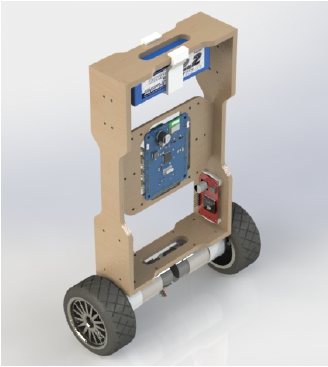
\includegraphics[scale=0.8]{EstadoArte/REF2}
    \caption{Protótipo renderizado
    \citep{JVM:17}.}
    \label{fig:estadoArte_REF2}
\end{figure}

Por último, o artigo de \cite{ME:18} propôs a implementação de um controlador LQR. A modelagem do sistema foi feita utilizando equações lagrangianas e, depois que encontrou uma equação não linear para o sistema, linearizou a mesma e passou para a forma de espaço de estados, chegando assim nas matrizes A, B, C e D. Aplicou a essas matrizes a propriedade de controlabilidade e observabilidade, concluindo assim, que é um sistema controlável e observável. O pêndulo invertido sobre duas rodas, é um sistema de uma única entrada e múltiplas saídas (SIMO). Dessa forma, para lidar com um tipo de sistema desses é mais simples com o LQR baseado pelo controle de velocidade como propôs o autor. Para utilizar esse controlador, é necessário encontrar um vetor de ganhos $K$ e consequentemente, minimizará a função de custo $J$. Na Figura (\ref{fig:estadoArte_REF3.1}) é mostrada a implementação do controlador LQR.
\begin{figure}[H]
    \centering
    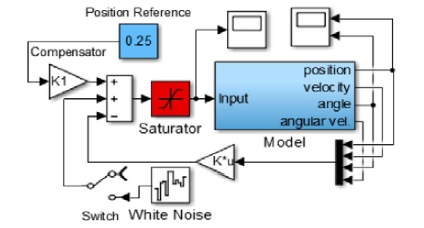
\includegraphics[scale=0.85]{EstadoArte/REF3_1.PNG}
    \caption{Implementação do controlador LQR
    \citep{ME:18}.}
    \label{fig:estadoArte_REF3.1}
\end{figure}

O filtro que foi implementado também foi o complementar, que nada mais é do que um filtro passa-baixas para o acelerômetro e um filtro passa-altas para o giroscópio. As principais variáveis que foram medidas ou estimadas foram: a posição da estrutura, $\theta$, a velocidade angular, $\dot{\theta}$ e, velocidade da roda, $\omega$. O protótipo montado pode ser visto na Figura (\ref{fig:estadoArte_REF3_2}). 
\begin{figure}[H]
    \centering
    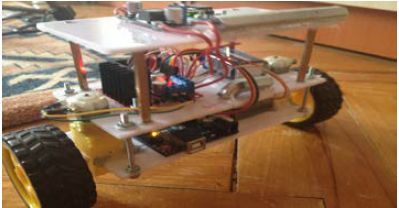
\includegraphics[scale=0.8]{EstadoArte/REF3_2}
    \caption{Planta física construída
    \citep{ME:18}.}
    \label{fig:estadoArte_REF3_2}
\end{figure}

\section{Fundamentos Clássicos da Mecânica}\label{sec:FundamentoClassicosMecanica}

O sistema em estudo conforme já citado é descrito como instável e não linear. Porém para encontrar as equações de movimento que regem o sistema, é preciso escolher algum tipo de método. Para o trabalho em questão, escolheu-se representar o sistema por meio da segunda lei de Newton descrita como sendo
\begin{equation}\label{SegundaLeiNewton}
    \sum \overrightarrow{F_i} = m\overrightarrow{a}
\end{equation}

\begin{equation}\label{SegundaLeiNewtonRotacao}
    \sum \tau_{iz} = J\alpha_z 
\end{equation}
em que os termos do lado esquerdo das Equações (\ref{SegundaLeiNewton}) e (\ref{SegundaLeiNewtonRotacao}) representam todas as forças $(F_i)$ e torques $(\tau)$ que atuam sobre o sistema. Já no lado direito da Equação (\ref{SegundaLeiNewton}), temos a massa total do corpo representada no centro de massa $(m)$ e todas as acelerações lineares $(a)$. Na Equação (\ref{SegundaLeiNewtonRotacao}), as acelerações agora são as angulares representas por $(\alpha_z)$ e o momento de inércia $(J)$ é dado como sendo
\begin{equation}
    J = \sum m_ir_i^2
\end{equation}
em que $m_i$ é a massa e $r$ a distância do objeto até o eixo de rotação.

Um outro fundamento que precisa ser descrito aqui é o cálculo do centro de gravidade (CG) ou centro de massa (CM) de um corpo. Para um sistema tridimensional pode-se definir um vetor posição desse sistema. Sendo uma partícula com coordenadas $x_i$, $y_i$ e $z_i$ seu vetor posição $\overrightarrow{r}$ é definido por
\begin{equation*}\label{eq:eqVetorPosicaoCentroMassa}
    \overrightarrow{r} = x_{cm}\hat{i} + y_{cm}\hat{j} + z_{cm}\hat{k}
\end{equation*}
no qual os vetores $\hat{i}$, $\hat{j}$, $\hat{k}$ são unitários e apontam na direção dos eixos $x$, $y$ e $z$ respectivamente. E finalmente, o cálculo da posição do centro de massa de um sistema de partículas é definido como
\begin{equation}
    \overrightarrow{CM} = \frac{1}{M} \sum\limits_{i=1}^{n} m_i\overrightarrow{r}_i
\end{equation}
em que $M$ é a massa total do sistema.

\section{Linearização}\label{sec:Linearizacao}

Como já dito, o sistema trabalho aqui neste traalho é de natureza não linear. Assim, para que as técnicas clássicas de controle ou mesmo algumas de controle moderno sejam utilizadas nos mesmos é preciso tratá-los por aproximações linearizantes.

Segundo \cite{Ogata}, um sistema para ser denominado de não linear é preciso que o princípio da superposição falhe ao ser aplicado nele. Dessa forma, caso tente obter uma resposta do sistema aplicando duas entradas simultâneas considerando as mesmas individualmente e somando-se os resultados, essa resposta não será válida.

Um sistema representado no espaço de estados é definido por \cite{Hespanha} da seguinte maneira
\begin{equation}\label{eq:DefinicaoSS}
    \begin{array}{cc}
         & \dot{x} = f(x,u) \\[6pt]
         & y = g(x,u)
    \end{array}{}
\end{equation}{}
sendo x $\in \mathbb{R}^{n}$ , y $\in \mathbb{R}^{m}$ e u $\in \mathbb{R}^{k}$.

\subsection{Ponto de equilíbrio}

Para se obter uma aproximação linear de um sistema não linear, é preciso, primeiramente, determinar os pontos de equilíbrio do sistema. A determinação dos pontos de equilíbrio é feito quando se iguala o termo diferencial da Equação (\ref{eq:DefinicaoSS}).

Pela definição de \cite{Hespanha}, têm-se que um par de pontos $(x^{eq},u^{eq})$ $\in$ $\mathbb{R}^n$ x $\mathbb{R}^k$ que pode ser chamado de ponto de equilíbrio de (\ref{eq:DefinicaoSS}) caso $f(x^{eq},u^{eq}) = 0$. A solução de (\ref{eq:DefinicaoSS}) é visto abaixo. 
\begin{equation}
    u(t) = u^{eq}, ~~~~~ x(t) = x^{eq}, ~~~~~ y(t) = y^{eq} := g(x^{eq},u^{eq}), ~~~~~~~~~~ \forall t \ge 0
\end{equation}{}

\subsection{Linearização em torno de um ponto de equilíbrio}\label{subsec:linearizacaoPontoEquilibrio}

De acordo com \cite{Hespanha}, a linearização do sistema em série de Taylor pode ser representado por matrizes Jacobianas, conforme descrito a seguir.

\begin{equation}\label{eq:MatrizesLineares}
    \begin{array}{cc}
         &  A := \dfrac{\partial f(x^{eq},u^{eq})}{\partial x}, ~~~~~~ B := \dfrac{\partial f(x^{eq},u^{eq})}{\partial u},\\[15pt]
         & C := \dfrac{\partial g(x^{eq},u^{eq})}{\partial x}, ~~~~~~ D := \dfrac{\partial g(x^{eq},u^{eq})}{\partial u}
    \end{array}{}
\end{equation}{}

Assim, o sistema linear invariante no tempo (LTI), no espaço de estados, linearizado em torno de um ponto de equilíbrio $(x^{eq},u^{eq})$, é dado por:

\begin{equation}
    \begin{array}{cc}
         &  \dot{\delta x} = A\delta x + B\delta u \\[6pt]
         &  \delta y = C\delta x + D\delta u
    \end{array}{}
\end{equation}{}
em que os termos $\dot{\delta x}(t), \delta{y}(t)$ e $\delta u(t)$ para todo $t \ge 0$ é descrito como
\begin{equation}
    \dot{\delta x}(t) := x(t) - x^{eq}, ~~~~~ \delta y(t) := y(t) - y^{eq}, ~~~~~ \delta u(t) := u(t) - u^{eq} 
\end{equation}{}


\section{Sistema em Espaço de Estados}\label{sec:EspacoEstados}

A representação no espaço de estados garante uma maior facilidade de soluções de um modelo matemático e de um sistema físico, já que a mesma pode relacionar um conjunto de variáveis de entradas, saídas e de estados por meio de equações diferenciais de primeira ordem. A representação fornece de maneira prática as soluções do sistema, por adotar notações matriciais quando o sistema dinâmico é linear e invariante no tempo.

\subsection{Caso contínuo no tempo}

No caso contínuo no tempo, um sistema representado no espaço de estados de acordo com \cite{Hespanha} pode ser descrito como
\begin{equation} \label{eq:SSContinuo}
    \begin{array}{cc}
         & \dot{x}(t) = A(t)x(t) + B(t)u(t) \\[6pt]
         & y(t) = C(t)x(t) + D(t)u(t)
    \end{array}{}
\end{equation}{}
no qual os sinais $u$, $y$ e $x$ das Equação (\ref{eq:SSContinuo}) são chamados de entrada, saída e de estados respectivamente e definidos por
\begin{equation*}
    \begin{array}{c}
        u:[0,\infty] \rightarrow \mathbb{R}^k, ~~~~~~~
        x:[0,\infty] \rightarrow \mathbb{R}^n, ~~~~~~~
        y:[0,\infty] \rightarrow \mathbb{R}^m
    \end{array}{}
\end{equation*}{}

Sendo o sistema representado pela Equação (\ref{eq:SSContinuo}) linear e as matrizes A(t), B(t), C(t) e D(t) constantes $\forall t \ge 0$, o sistema  é chamado de linear invariante no tempo (LTI). Assim, pode-se simplificar a representação no caso contínuo
\begin{equation}\label{eq:SSContinuoLTI}
    \begin{array}{cc}
         & \dot{x}(t) = Ax(t) + Bu(t) \\[6pt]
         & y(t) = Cx(t) + Du(t)
    \end{array}{}
\end{equation}{}

As dimensões das matrizes $A$, $B$, $C$ e $D$ das Equações (\ref{eq:SSContinuo}) e (\ref{eq:SSContinuoLTI}) são as mesmas e são definidas como sendo
\begin{equation*}
    \begin{array}{cc}
    &    A \in \mathbb{R}^{n \times n} ~~~~~~~
         B \in \mathbb{R}^{k \times m}  \\[6pt]
    &    C \in \mathbb{R}^{l \times n} ~~~~~~~
         D \in \mathbb{R}^{l \times m}
    \end{array}{}
\end{equation*}{}


\subsection{Caso discreto no tempo}

As aplicações de forma geral são feitas utilizando microcontroladores ou algum dispositivo digital. Sendo assim, para aplicações desse tipo, faz-se necessário a discretização do sistema. 

\cite{Chen} afirma que a representação discreta do sistema no espaço de estados é descrita como
\begin{equation}
    \begin{array}{cc} \label{eq:SSDiscretoLTI}
         & x_{k+1} = A_dx_k + B_du_k \\[6pt]
         & y_k = C_dx_k + D_du_k
    \end{array}{}
\end{equation}{}
em que a variável $t=kT$ com $k=0,1,2,..,k_f$ e $T$ o período de amostragem do sistema. O período é escolhido de forma a ser o menor possível, ou seja, o máximo que o microcontrolador consegue trabalhar. As matrizes $A_d$, $B_d$, $C_d$, $D_d$ são descritas como se segue bem como a solução para $A_d$ e $B_d$ \citep[p. 91]{Chen}
\begin{equation}\label{eq:MetodoDiscretizacao}
    A_d = e^{AT} ~~~~~ B_d = \left(\int_{0}^{T} e^{A\tau} \, d\tau\right)B~~~~~  C_d = C ~~~~~ D_d = D    
\end{equation}


\section{Realimentação de Estados}

Uma das formas de se implementar controladores por meio da representação no espaço de estados é por meio da realimentação de estados, no qual utiliza-se os próprios estados do sistema com um fator multiplicativo (ganho) para gerar o sinal de controle. Para ter acesso a todos os estados da planta deve-se ter sensores para cada um dos estados do sistema. Como na maioria das aplicações reais isso não ocorre, pois implica em um custo elevado, faz-se necessário a implementação de um sistema que irá estimar os estados (observador) e assim, o sinal de controle passará a ser com relação a esses estados estimados. Contudo, para realizar a construção de um observador ou mesmo fazer o controle do sistema, deve-se, primeiramente, testar o sistema com métodos matemáticos que informam tais capacidades. Dito isso, os critérios são apresentados a seguir para um sistema discreto
\begin{equation}\label{eq:SSDiscretoLTI2}
    \begin{array}{cc}
         &  x_{k+1} = A_dx_k + B_du_k \\[10pt]
         &  y_k = C_dx_k + D_du_k
    \end{array}{}
\end{equation}{}

\subsection{Controlabilidade}

De acordo com \cite{Hespanha}, para saber se o sistema é controlável ou não, utiliza-se as matrizes $A_d$ e $B_d$ da equação de estados de (\ref{eq:SSDiscretoLTI2}). O critério para determinar a controlabilidade é demonstrado como sendo
\begin{equation}\label{eq:Controlabilidade}
\mathbb{C} := \left[\begin{array}{ccccc}
        B_d & A_dB_d & A_d^2B_d & \dots & A_d^{n-1}B_d
     \end{array}\right]_{n\times(kn)} 
\end{equation}{}

A partir do critério (\ref{eq:Controlabilidade}) pode-se determinar se o sistema em questão poderá ou não ser controlável. Segundo \cite{Ogata}, para que o sistema seja controlável é preciso que o determinante da matriz (\ref{eq:Controlabilidade}) seja diferente de $0$, ou seja, que tenham vetores linearmente independentes (LI) e assim, posto $n$.

\subsection{Observabilidade}

Como não haverá medições diretas de todos os estados, será necessário a utilização de um observador como já mencionado. O mesmo irá estimar o valor dos estados que faltam e assim a lei de controle da realimentação será baseado neles. 

Contudo, nem todos os sistemas são observáveis, dessa forma é preciso garantir que o sistema deste trabalho seja observável. De acordo com \cite{Hespanha}, o critério no qual testa-se o sistema será observável ou não é mostrado como sendo
\begin{equation}\label{eq:Observabilidade}
\mathbb{O} := \left[\begin{array}{c}
        C_d ~ \\ C_dA_d ~ \\ C_dA_d^2 ~ \\ \vdots ~ \\ C_dA_d^{n-1}
    \end{array}\right]_{(kn) \times n}
\end{equation}\\

A análise da matriz (\ref{eq:Observabilidade}) é dual ao critério de controlabilidade. Para que o sistema seja observável é preciso que os vetores sejam LI, ou seja, que tenham posto ($\textit{rank}$) igual a $n$.

\section{Controlador Linear Gaussiano Quadrático (LQG)}\label{sec:MetodologiaControladorLQG}

De acordo com \cite{Steven:17}, o controlador LQG é constituído por um estimador quadrático linear (LQE) ou mais popularmente denominado de Filtro de Kalman, ou seja, um observador no qual os estados estimados são realimentados através de ganhos ótimos projetados por meio do regulador linear quadrático (LQR). A Figura (\ref{fig:controladorLQG}) apresenta como deve ser o \textit{design} de um controlador LQG.
\begin{figure}[H]
    \centering
    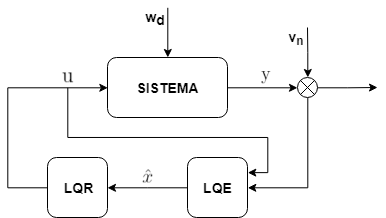
\includegraphics[scale=0.75]{Fundamentos/LQG}
    \caption{Estrutura de um controlador LQG.}
    \label{fig:controladorLQG}
\end{figure}

\subsection{Regulador Linear Quadrático  (LQR)}\label{subsec:MetodologiaControladorLQR}

O LQR possui como principal característica a garantia de estabilidade em malha fechada, um alto grau de robustez do sistema controlado proporcionado ao mesmo margem de ganho infinita e margem de fase $\pm 60^\circ$ \citep{Fernandes:14}. Contudo, se faz necessário conhecer todos os estados do sistema para se trabalhar com este regulador. Dessa maneira, é usual utilizar este controlador juntamente com um estimador tal como o LQE.

Para encontrar o ganho ótimo do LQR, considera-se o seguinte sistema no tempo discreto.
\begin{equation}
    \begin{array}{cc}
         &  x_{k+1} = A_dx_k + B_du_k \\[6pt]
         &  y_k = C_dx_k
    \end{array}{}
\end{equation}{}

Assume-se que $x(0) = x_0$ e $k = 0, 1, 2,\dots,k_f$. De acordo com \cite{Sage}, a função de custo a ser minimizada é dada por:
\begin{equation}\label{eq:FuncaoCustoLQR}
    J = \frac{1}{2}||x_{k_f}||^2_S + \frac{1}{2}\sum_{k=0}^{k_f-1} \{||x_k||^2_Q + ||u_k||^2_R\}
\end{equation}{}

A matriz $Q \in \reais^{nxn}$ é uma matriz positiva semi-definida e $R \in \reais^{mxm}$ é uma matriz positiva definida. Essas matrizes são responsáveis pela ponderação dos estados e o sinal de controle do sistema. De acordo com \cite{Matos:08}, essas matrizes são escolhidas da seguinte forma:
\begin{equation*}
    \begin{array}{cc}
         &  Q = C_d^TC_d\\[6pt]
         &  R = \rho \I_{mxm}, ~~~ \rho > 0.
    \end{array}{}
\end{equation*}{}

Conforme \cite{Sage}, a equação Hamiltoniana é dada como se segue.
\begin{equation}\label{eq:Hamiltoniana}
    H_k = \frac{1}{2}x_k^TQx_k + \frac{1}{2}u_k^TRu_k + \lambda_{k+1}^T[A_dx_k + B_du_k]
\end{equation}{}

Caso o par $(A_d,B_d)$ seja controlável e o par $(A_d,C_d)$ observável, a lei de controle ótimo que minimiza a equação de custo (\ref{eq:FuncaoCustoLQR}) é dada por:
\begin{equation}\label{eq:LeiControleLQR}
    u_k = -Kx_k
\end{equation}{}
em que a matriz $K \in \mathbb{R}^{mxn}$ de ganhos ótimos do controlador LQR é definida como se segue
\begin{equation}\label{eq:GanhoLQR}
    K = (R + B_d^TPB_d)^{-1}B_d^TPA_d
\end{equation}{}
no qual a matriz simétrica $P \in \mathbb{R}^{nxn}$ é conseguida após solucionar a equação de Riccati de forma recursiva como segue
\begin{equation}\label{eq:RiccatiLQR}
    P_{k+1} = Q + A^TP_kA_d - A_d^TP_kB_d(R + B_d^TP_kB_d)^{-1}B_d^TP_kA_d
\end{equation}{}

\subsection{Estimador de Estados Quadrático (LQE)}\label{sec:MetodologiaFiltroKalman}

\cite{Sundin:12} afirmam que os o filtro capaz de fazer a estimação da derivada do giroscópio é o Filtro de Kalman. O Filtro de Kalman surgiu da teoria de otimização e é um estimador ótimo para sistemas que possuem distúrbios e apresentam características de distribuição normal de ruído branco. O filtro modela o comportamento do sensor e isso inclui o $\textit{bias}$ que possa vir a ter, o que dá uma boa estimativa do ângulo e do $\textit{bias}$ do giroscópio, que melhora a taxa angular uma vez que o mesmo pode ser removido. A Figura (\ref{fig:estimadorLQE}) apresenta a estrutura do filtro no tempo discreto.
\begin{figure}[H]
    \centering
    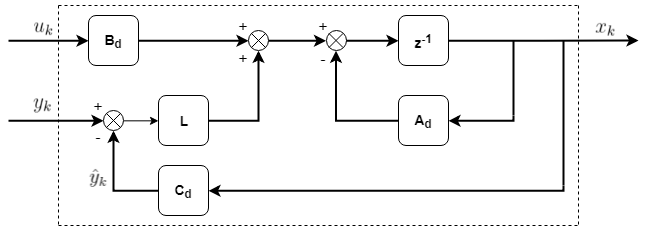
\includegraphics[scale=0.6]{Fundamentos/Kalman}
    \caption{Estrutura do Filtro de Kalman discreto em Espaço de Estados. Adaptado de \cite{Steven:17}.}
    \label{fig:estimadorLQE}
\end{figure}

O ganho do estimador ótimo quadrático linear se baseia no desempenho do observado projetado com a presença de erro de medição e ruído de processo. Logo, a cada tempo que passa o ganho do filtro de Kalman vai sendo atualizado. Primeiramente, para realizar o projeto desse estimador considera-se o seguinte sistema
\begin{equation}\label{eq:SistemaLQE}
    \begin{array}{cc}
         &  x_{k+1} = A_d x_k + B_d u_k + w_k\\[6pt]
         &  y_k = C_dx_k + v_k
    \end{array}{}
\end{equation}{}
em que o ruído $w_k$ e o erro de medição $v_k$ são sequências aleatórias de ruído branco gaussiano com média zero \cite[p. 231]{Sage}. Sendo assim, temos
\begin{equation*}
    \mathbb{E}\{w_k\} = 0 ~~~ \text{e} ~~~ \mathbb{E}\{v_k\} = 0 
\end{equation*}{}
em que $\mathbb{E}\{\}$ é conhecido como expectância ou valor esperado. A correlação por se tratar de ruído branco é zero 
\begin{equation*}
    cov\{w_iw_j^T\} = 0 ~~~ \text{e} ~~~ cov\{v_iv_j^T\} = 0 ~~~ \text{para} ~~~ i \ne j
\end{equation*}{}
e a covariância é definida por
\begin{equation*}
    cov\{w_kw_k^T\} = Q_o ~~~ \text{e} ~~~ cov\{v_kv_k^T\} = R_o
\end{equation*}{}

A principal tarefa da otimização é determinar uma matriz de ganhos que minimizará a variância da estimação do erro, que é denotado por $G_k$
\begin{equation}\label{eq:VarianciaEstimacao}
    G_k = \mathbb{E} \{(x_k-\hat{x}_k)(x_k-\hat{x}_k)^T\}
\end{equation}{}

Segundo \cite{Steven:17}, um estimador produz uma estimação dos estados $x_k$ conhecida como $\hat{x_k}$ caso conheça a saída medida $y_k$ provinda de um sensor e o sinal de entrada $u_k$. Caso o sistema seja observável, é possível construir o filtro a partir do ganho $L$ como se segue
\begin{equation}\label{eq:DinamicaEstimadorLQE}
    \begin{array}{cc}
        &  \hat{x}_{k+1} = A_d \hat{x}_k + B_d u_k + L_k(y_k - \hat{y}_k) \\
        &  \hat{y}_k = C_d\hat{x}
    \end{array}{}
\end{equation}{}
sendo que a saída $\hat{y}_k$ é a predição da expectativa da saída do sensor baseada no estados estimados $\hat{x}_k$. Manipulando a Equação
(\ref{eq:DinamicaEstimadorLQE}), encontra-se uma expressão para $\hat{x}_{k+1}$.
\begin{align}
     \hat{x}_{k+1} & = (A_d - LC_d)\hat{x}_k + B_du_k + Ly_k \nonumber \\ 
                   & = (A_d - LC_d)\hat{x}_k + \left[\begin{array}{cc}
                                            B_d & L
                                            \end{array}{}\right]    \left[\begin{array}{cc}
                                        u_k\\
                                        y_k
                                    \end{array}{}\right]
\end{align}
assim, as matrizes $A_f$ e $B_f$ do filtro de Kalman são:
\begin{align}\label{eq:MatrizesFiltroKalman}
    \begin{array}{cc}
        A_f = \left(\begin{array}{c}                   
                    A_d - LC_d
                \end{array}\right) ~~~~~~~~~~~
        B_f = \left[\begin{array}{cc}
                 B_d & L 
              \end{array}\right]
    \end{array}{}
\end{align}{}

De acordo com \cite{Kim:13}, o ganho $L$ do filtro de Kalman é um vetor pertencente aos números reais e de dimensão n$\times$1 e é definido pela seguinte expressão
\begin{equation}\label{eq:Ganho1LQE}
    L = A_dS_kC_d^T(C_dSC_d^T + R_o)^{-1}
\end{equation}{}
na qual a matriz S é obtida quando soluciona-se a equação de Riccati
para a equação de diferenças. A expressão que precisa-se solucionar e que fará com que o ganho $L$ seja ótimo é descrita como
\begin{equation}\label{eq:MatrizMinimizaçãoLQE}
    S_{k+1} = Q_o + A_dS_kA_d^T - A_dS_kC^T(C_dS_kC_d^T + R_o)^{-1}C_dS_kA_d^T
\end{equation}{}
em que $Q_o$ é uma matriz positiva definida e $R_o > 0$ são especificados como parâmetros de projeto, considerando a condição inicial $S_0 = 0$.










\begin{comment}

\section{Filtros}\label{sec:Filtros}

Em grande parte de sistemas que utilizam de sensores necessitam de algum tipo de filtro. E nesta seção dois filtros testados e aplicados no sistema serão explicados.

Primeiramente, para um boa estimação da inclinação do pêndulo é necessário que os sinais de leitura do acelerômetro e do giroscópio sejam fundidos com objetivo de criar um novo sinal mais estável e fidedigno. Segundo \cite{Sundin:12}, os sensores possuem diferentes propriedades que afetam a estimação do ângulo de diferentes maneiras. Abaixo é listado as principais de cada.
\begin{itemize}
    \item \textbf{Acelerômetro}: o acelerômetro tem uma boa leitura da inclinação da estrutura quando outras forças não atuam sobre ele tais como movimentos lineares. Para se conseguir uma estimativa correta é necessário que apenas a força da gravidade esteja atuando sobre o sensor ou então o mesmo não retornará uma leitura fiel do ângulo.

    \item \textbf{Giroscópio}: o giroscópio tem uma boa estimativa do ângulo \textit{pitch}, $\theta$, realizando a integral da saída de interesse, ou seja, da inclinação do sistema. Esse ângulo não é afetado por forças lineares pela movimentação do robô mas o sensor pode ter sua leitura comprometida caso o mesmo apresente algum \textit{bias} (ou \textit{offset}) que fará com que sua leitura não seja a verdadeira.
\end{itemize}

Utilizando os conhecimentos a respeito de filtros os mesmos podem ser utilizados para obter uma resposta mais confiável então da leitura do ângulo. Dessa maneira, abaixo será descrito dois filtros utilizados no sistema que fazem a fusão dos sensores.

\subsection{Filtro Complementar}

O filtro complementar é em sua maior parte utilizada em projetos $\textit{hobbistas}$ por ser simples e um bom filtro de fusão para dois sensores. O filtro possui fácil implementação e de ajuste experimental e demanda pouco poder de processamento \citep{Sundin:12}. Por ser formado por dois fitros, passas altas e passas baixas, cada um atua em um sensor, sendo que o primeiro atua no giroscópio e o segundo no acelerômetro. O ângulo $\theta$ é dado pela seguinte maneira
\begin{equation}
    \theta_k = (1 - \alpha)(\theta_{k-1} + \dot{\theta}_{k,gyro}dt) + \theta\alpha_{k,acc}
\end{equation}
em que $dt$ é o tempo de amostragem e $\alpha$ é a constante do filtro. Então, para extrair o que este filtro tem de melhor, é necessário ajustar a contante $\alpha$ até que o resultado seja bom, o que faz a constante de tempo do filtro alterar e consequentemente o $\textit{bias}$ do giroscópio é removido. Por mais que este filtro pareça ser excelente por todas as vantagens apresentadas, o mesmo apresenta desvantagens tal como não saber o $\textit{bias}$ real do giroscópio e assim dará apenas uma boa estimativa do ângulo.

\section{PWM}\label{sec:PWM}
Uma vez que o sistema será alimentado por uma bateria, a mesma fornece uma tensão constante e para poder variar a velocidade dos motores é preciso controlar a tensão. Assim, para esta modulação foi utilizado uma técnica simples de baixas perdas energéticas e que tem suporte do \textit{hardware} e \textit{software} no Arduino \textbf{CITAR SUSAN}. Dessa forma, a energia é drenada da bateria e ligada e desligada pelo controlador dos motores. Devido a inércia elétrica, a tensão não atingirá o zero volts e nem ao máximo entre cada período de comutação, mas em vez disso, estará próximo da média resultante dependendo do ciclo de trabalho (\textit{Duty Cicle}) $D$. A tensão de saída do PWM é descrita como
\begin{gather}
    U = \frac{1}{T}\int_{0}^{T} f(t)\, dt
\end{gather}
e $f(t)$ é uma função de pulso descrita como sendo
\begin{equation}
f(t) = 
    \left \{
        \begin{array}{cc}
            U_{max}, & \mbox{se } 0 < t \leq D\times T \\
            0      , & \mbox{se } D\times T < t \leq T \\
        \end{array}
    \right.
\end{equation}
que por sua vez produz uma tensão média que pode ser calculada como
\begin{equation}
    U = D \times U_{max}
\end{equation}

A Figura (\ref{fig:PWM}) explica graficamente a função $f(t)$.
\begin{figure}[!htb]
    \centering
    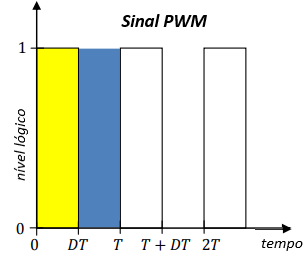
\includegraphics[scale=0.8]{Metodologia/PWM}
    \caption{Gráfico que demonstra o funcionamento do sinal PWM. A parte colorida de amarelo é o sinal em alta ou quando o sinal está ligado e em azul o oposto.}
    \label{fig:PWM}
\end{figure}

\end{comment}

